% Describe the approaches you have used to evaluate that the solution you have 
% designed in \Cref{ch:design} and executed in \Cref{ch:implementation} actually 
% solves the problem identified in \Cref{ch:introduction}.

% While you can discuss unit testing etc. you have carried here a little bit, 
% that is the minimum. You should present data here and discuss that. This might 
% include \emph{e.g.} performance data you have obtained from benchmarks, survey 
% results, or application telemetry / analytics. Tables and graphs displaying this 
% data are good.
In this chapter, we evaluate our implementation with respect to testing and
the results of our benchmarks. 

\section{Testing}\label{eval:testing}
We implement tests for all major components of our system based on our approach 
described in Section \ref{design:testing}. These tests have been scrutinised to ensure 
they test the expected behaviour of each component, especially those 
that are based on protocols from the literature. Readers who are interested can 
run these tests using the \texttt{cargo test} command, to verify that all tests pass. 
Using code coverage analysis, we also ensure that we do not miss any important test 
cases and that we are testing as much of our code and as many edge cases as possible.
We use the following command to generate a code coverage report:

\begin{lstlisting}[language=bash]
  cargo llvm-cov --open --ignore-filename-regex libs/stacksig-compiler/src/rot256
\end{lstlisting}

\begin{figure}[t]
  \centering
  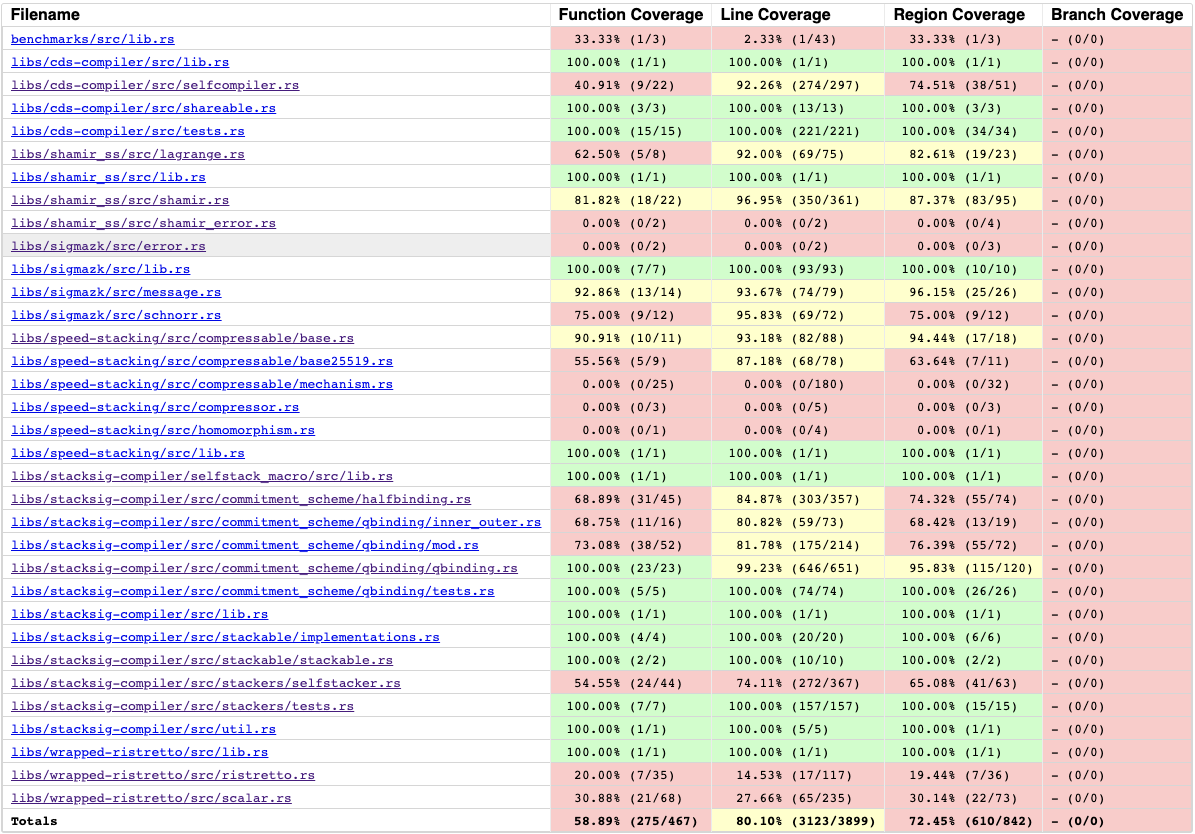
\includegraphics[width=\linewidth]{../assets/code-coverage.png}
  \caption{Code coverage of our project}
  \label{fig:coverage}
\end{figure}

We exclude the files within the \texttt{rot256} directory as those are related to Hall-Andersen's implementation \cite{MHAStackSig}. The code coverage report produced by this command can be seen in Figure \ref{fig:coverage}. 

From this report, we observe that we have only 58.89\% function 
coverage (we only test 58.89\% of the functions in our project), 80.10\% line 
coverage, and 72.45\% region coverage\footnote{Regions are blocks of code with 
respect to the compiler -- these can be multiple lines of code with no control flow 
or a single line of code. These regions for Rust are determined by LLVM. \cite{llvm-cov-explain}}. These numbers may appear to be low but upon closer inspection,
we observe the following:
\begin{enumerate}
  \item \textbf{Functions}: the majority of the functions that are not tested are either
  \begin{itemize}
    \item Getter and setter functions for classes (structs in Rust). These functions 
    simply return or set a value within the class, and are not tested as they are very simple. 
    \item or derived traits \cite{rust-book-derived-traits} in Rust. These are functions that are automatically generated according to "macros", which allow users to derive the implementation of specific interfaces for their classes automatically. These functions are not tested as they are automatically generated by the compiler. 
  \end{itemize}
  \item \textbf{Lines}: A portion of these lines include those for the Speed Stacking 
  compiler that we are still working on \cite{SpeedStacking}. These could not be 
  easily removed from the code coverage report, and affect the line coverage statistics.
  Additionally, many of these lines are automatically generated by the compiler from 
  derived traits. 
  \item \textbf{Regions}: While most regions are affected by the same reasons as functions and lines, it should be noted that there are some regions that should be 
  tested more thoroughly but are not. These regions are related to error-producing 
  branches of code, which should be tested to ensure that our implementation handles 
  errors correctly. The bulk of these regions are located in our implementation of 
  Shamir's secret sharing scheme. However, due to the low priority, and time constraints 
  of this project, we have not been able to test these cases thoroughly.
\end{enumerate}

Aside from these areas, all the main requirements of our compilers and respective 
software components are tested thoroughly. While it is ideal to achieve higher 
than 80\% code coverage in all categories, we believe that code coverage is useful in 
identifying potential areas of improvement for testing, but should not be used as the
sole metric for evaluating the quality of our tests. In fact, the code coverage report
was useful in highlighting that we previously did not implement a proper 
negative test for the CDS94 compiler as the block of code that returns false in 
the verification algorithm was not covered by any tests. This was subsequently fixed, 
improving the code coverage report marginally, but covering an important case 
for our compiler.

In summary, we assess that our quality and thoroughness of testing are sufficient 
for the scope of this project. However, we acknowledge that there is still room for
improvement in our testing, especially in the areas of error handling. 

\section{Benchmark Results}\label{eval:benchmarks}
In this section, we present the results of our benchmarks and discuss their 
implications. We have four benchmarks: two for the CDS94 compiler \cite{CDS94}, 
one for the Stacking Sigmas compiler \cite{StackingSigmas}, and one from Hall-Andersen's implementation \cite{MHAStackSig}. One of the two benchmarks for the CDS94 compiler compares 
the growth of the key metrics against the number of active clauses (instead of the number of clauses). We will first present and discuss the results regarding the 
growth in communication size across all benchmarks. After this, we will discuss
the results for the measurements of the growth in the computation time. In table \ref{tab:comm-size} and 
\ref{tab:comp-time}, we present the overall results of our benchmarks. These benchmarks were executed on an M1 MacBook Air (16GB) -- we provide the hardware specifications of our machine in Section \ref{sec:hardware-spec}. Note that the first row of Stacking Sigmas has no data as a result of a flaw in our current implementation of the q-binding scheme as mentioned in \ref{design:qbinding}.
\begin{table}[H]
  \centering\caption{Communication Size Results (in bytes)} 
  \label{tab:comm-size}
  \begin{tabular}{rcc}
    \toprule
    \textbf{Clauses} & \textbf{CDS94} & \textbf{Stacking Sigmas} \\
    \midrule
    2 & 224 & - \\
    4 & 416 & 256 \\
    8 & 800 & 320 \\
    16 & 1568 & 384 \\
    32 & 3104 & 448 \\
    64 & 6176 & 512 \\
    128 & 12320 & 576 \\
    256 & 24608 & 640 \\
    512 & 49184 & 704 \\
    1024 & 98336 & 768 \\
    2048 & 196640 & 832 \\
    4096 & 393248 & 896 \\
    8192 & 786368 & 960 \\
    \bottomrule
  \end{tabular}
\end{table}

\begin{table}[H]
\centering
\caption{Computation Time Results (in milliseconds)}
\label{tab:comp-time}
\begin{tabular}{rccccc}
\toprule
\textbf{Clauses} & \textbf{StackSig Prover} & \textbf{CDS Prover} & \textbf{StackSig Verifier} & \textbf{CDS Verifier} & \textbf{Rot256} \\
\midrule
2 & 0.3 & 0.081124 & 0.3 & 0.10955 & 3.4760 \\
4 & 0.64893 & 0.19991 & 0.64233 & 0.22346 & 7 \\
8 & 1.8222 & 0.45870 & 1.3788 & 0.47586 & 10.9 \\
16 & 4.2626 & 0.98115 & 2.8526 & 0.97444 & 15.021 \\
32 & 9.3257 & 2.1472 & 5.9700 & 2.0985 & 20.069 \\
64 & 19.616 & 5.0377 & 11.705 & 4.9214 & 37 \\
128 & 40.584 & 13.105 & 24.474 & 12.696 & 37.131 \\
256 & 82.243 & 37.381 & 47.087 & 36.691 & 54.213 \\
512 & 165.70 & 120.33 & 93.798 & 118.92 & 85 \\
1024 & 334.63 & 422.50 & 190.63 & 419.73 & 145.33 \\
2048 & 671.82 & 1572.9 & 375.45 & 1583.5 & 257.25 \\
4096 & 1359.1 & 6110.2 & 742.17 & 6081.9 & 482.62 \\
8192 & 2685.4 & 24141 & 1477.9 & 23884 & 932.34 \\
\bottomrule
\end{tabular}
\end{table}

\paragraph{Running benchmarks.} To run our benchmarks, we use the \texttt{cargo bench} command. To run the benchmarks for a specific compiler, we use the \texttt{{-}{-}bench} flag. Below we provide an example of how to run each benchmark available:
\begin{lstlisting}[language=bash]
  # run benchmark for CDS94 (as clauses increase)
  cargo bench --bench cds_benchmark 
  # run benchmark for CDS94 (as active clauses increase)
  cargo bench --bench cds_benchmark2 
  # run benchmark for Stacking Sigmas (as clauses increase)
  cargo bench --bench stacksig_benchmark 
  # run benchmark for Hall-Andersen's implementation (as clauses increase)
  cargo bench --bench rot256_benchmark
  # run all benchmarks available: requires a long time
  cargo bench
\end{lstlisting}

\subsection{Communication Size}\label{eval:comm}
We present two figures, Figure \ref{fig:cds_comm} and Figure \ref{fig:stacksig_comm},
for the CDS94 compiler and Stacking Sigmas compiler respectively. These figures 
show the growth in communication size for each compiler as the number of clauses
increases. Note that the $x$-axis of these figures is logarithmic. Therefore, a 
linear and logarithmic growth in communication size is represented by a quadratic and linear growth in the logarithmic scale respectively. 
\begin{figure}[h]
  \centering
  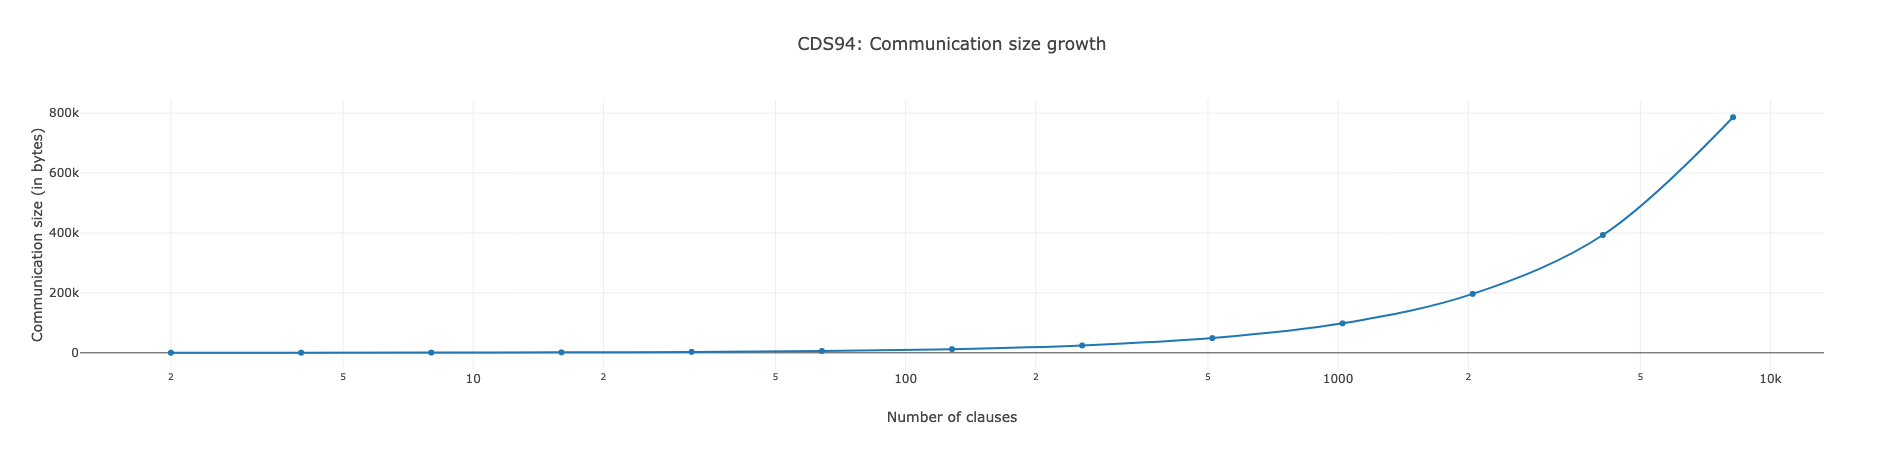
\includegraphics[width=\linewidth]{../assets/plots/cds_commsize.png}
  \caption{The growth in communication size for the CDS94 compiler. }
  \label{fig:cds_comm}  
\end{figure}

\begin{figure}[h]
  \centering
  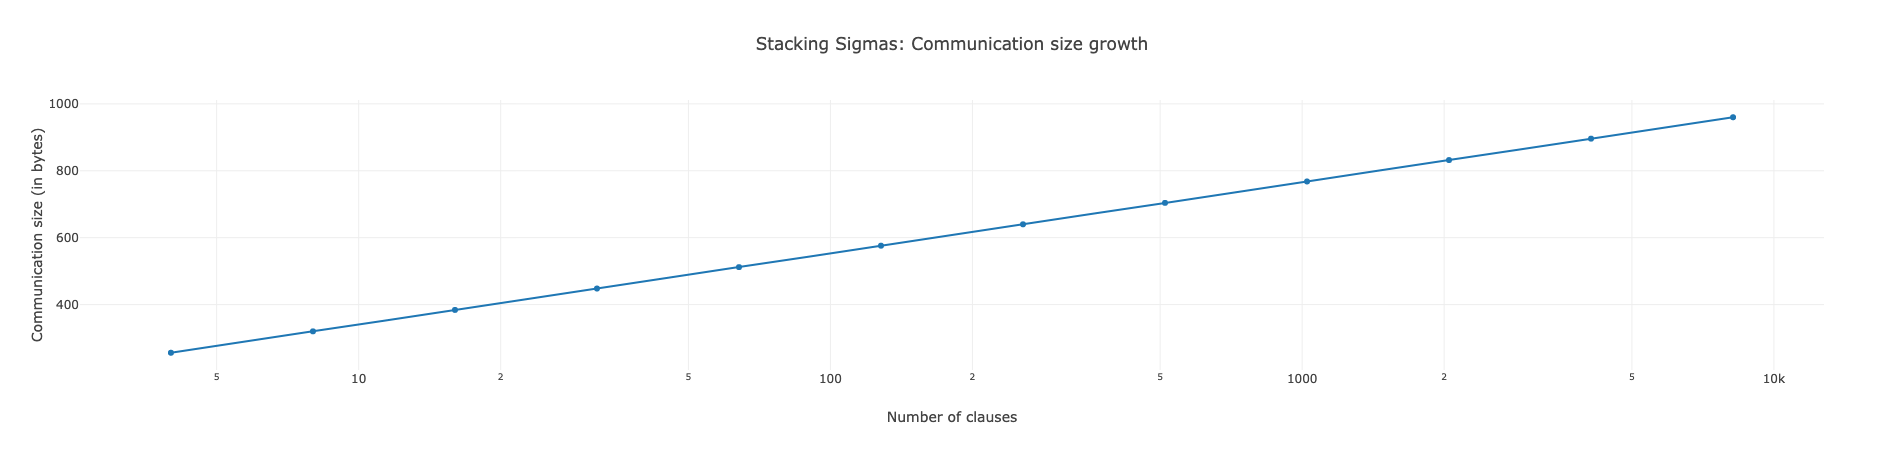
\includegraphics[width=\linewidth]{../assets/plots/ss_commsize.png}
  \caption{The growth in communication size for the Stacking Sigmas compiler. }
  \label{fig:stacksig_comm}
\end{figure}

In both cases, we point out that the communication size growth is consistent with 
the theoretical proofs of the respective compilers. This further validates our
implementation of the compilers. The expected growth in communication size for
the CDS94 compiler is linear, which appears as a quadratic growth with a 
logarithmic scale. Meanwhile, the equivalent for the Stacking Sigmas compiler is
a logarithmic growth, which appears as a linear growth in the logarithmic scale. 

With an increasing number of active clauses, but a constant number of clauses, 
the communication size for the CDS94 compiler is not expected to change. This is
because the number of active clauses does not affect the number of elements in the 
vector of messages sent by the prover. This is supported by the results in Figure
\ref{fig:cds_comm2}. This figure shows that the communication size for 512 
clauses is constant at 53.28KB, regardless of the number of active clauses.

\begin{figure}[h]
  \centering
  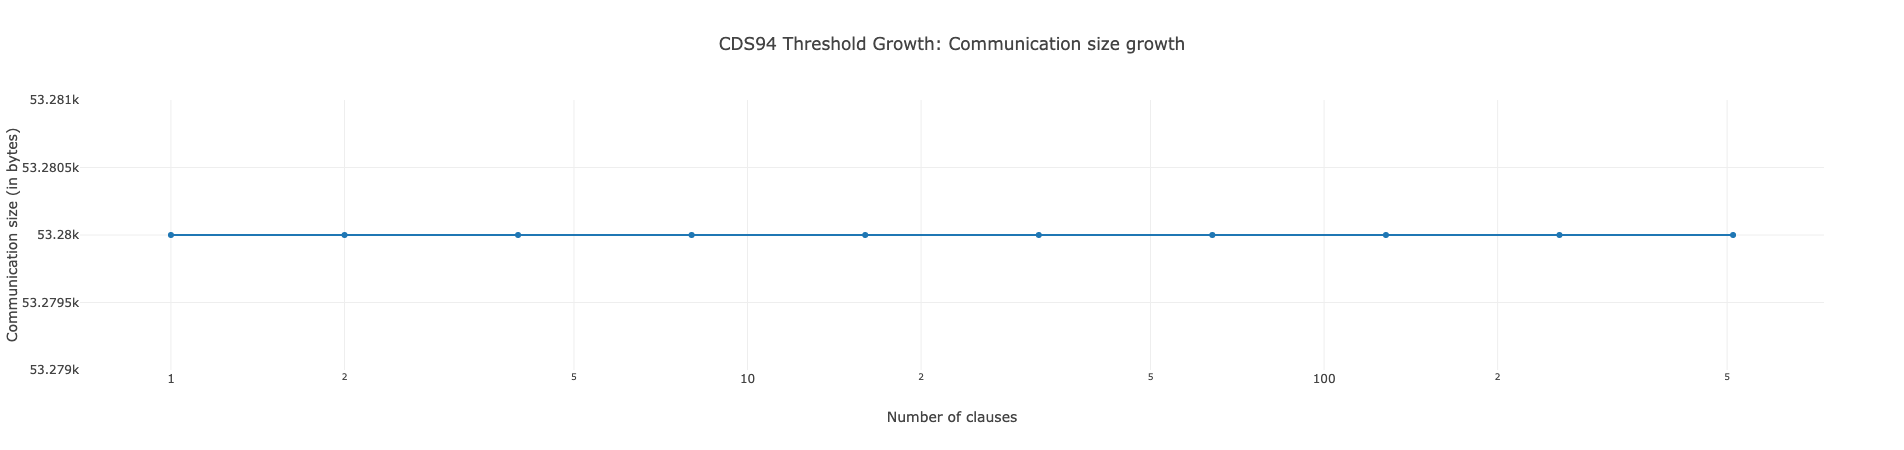
\includegraphics[width=\linewidth]{../assets/plots/cds2_threshold.png}
  \caption{The growth in communication size for the CDS94 compiler as the number of active clauses increases (total clauses = 512).}
  \label{fig:cds_comm2}
\end{figure}

We do not provide a similar figure for Hall-Andersen's implementation as the 
results are identical to Figure \ref{fig:stacksig_comm}. In conclusion, the 
observed growth in communication size is consistent with the theoretical
proofs of the respective compilers, further supporting the correctness of our
implementations, and also validating these proofs.

\subsection{Computation Time}\label{eval:time}
Firstly, we present the comparison between the prover and verifier running 
time for each compiler. 

\paragraph{CDS94 Prover vs Verifier.} In Figure \ref{fig:cds_vs}, we compare the 
prover and 
verifier running time in our implementation of \cite{CDS94}. From the figure, 
we observe that both running times are quadratic as 
the number of clauses increases. This is mainly because polynomial interpolation
using Lagrange is the bottleneck with a quadratic running time. This 
directly affects both the prover and verifier running times, as both the 
third-round protocol and the verification algorithm use this algorithm. 

\begin{figure}[H]
  \centering
  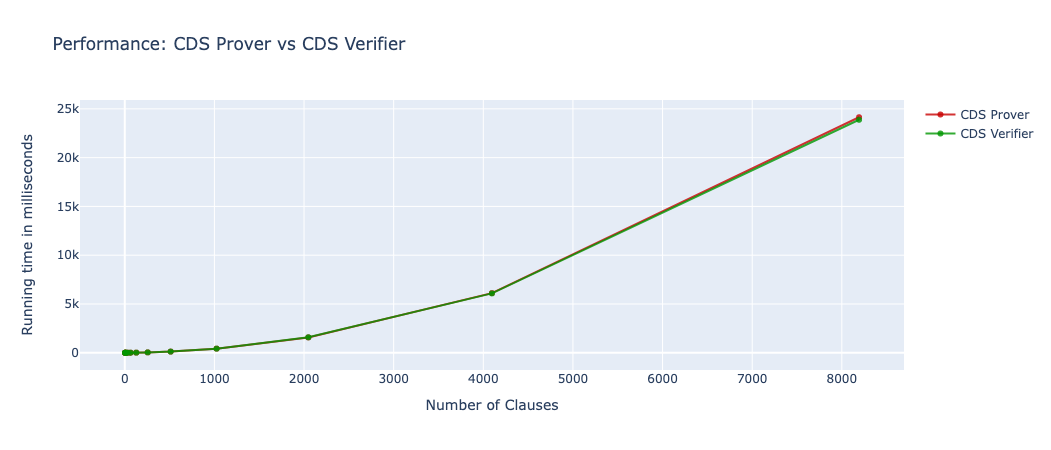
\includegraphics[width=\linewidth]{../assets/plots/cds_vs.png}
  \caption{A comparison of the prover and verifier running time of CDS94. }
  \label{fig:cds_vs}
\end{figure}

\begin{figure}[H]
  \centering
  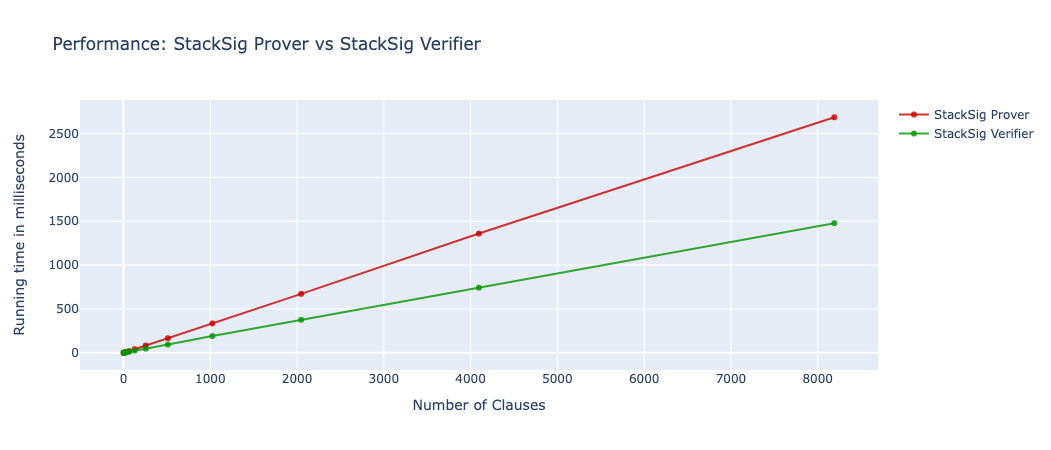
\includegraphics[width=\linewidth]{../assets/plots/ss_vs.png}
  \caption{A comparison of the prover and verifier running time of Stacking Sigmas.}
  \label{fig:stacksig_vs}
\end{figure}

\paragraph{Stacking Sigmas Prover vs Verifier.} In Figure \ref{fig:stacksig_vs}, we compare the prover and verifier running time
for the Stacking Sigmas compiler. The graph shows a linear growth in computation time 
for both the prover and verifier, which is expected. The computation time of the prover has 
a larger constant factor than that of the verifier. This is likely the case 
because the prover algorithms call the \textsf{Equiv} and \textsf{EquivCom} 
methods from the q-binding scheme, which are more computationally expensive than
the \textsf{Bind} method used in the verifier algorithm.

\paragraph{CDS94 vs Stacking Sigmas.} Next, we compare the prover algorithms of CDS94 and Stacking Sigmas. In Figure \ref{fig:provers_vs}, we see that up until 512 clauses, the CDS94 prover is more 
performant. However, due to the quadratic running time of the CDS94 prover, the 
Stacking Sigmas prover starts to outperform CDS94 after 512 clauses. 
Similarly in Figure \ref{fig:verifiers_vs}, where we compare the verifier algorithms 
across the two compilers, CDS94 is more performant when there are 256 or fewer clauses. 
 After which, Stacking Sigmas overtakes and takes less time to run. Note that both the 
$x$-axis and the $y$-axis are on the logarithmic scale. 

\begin{figure}[h]
  \centering
  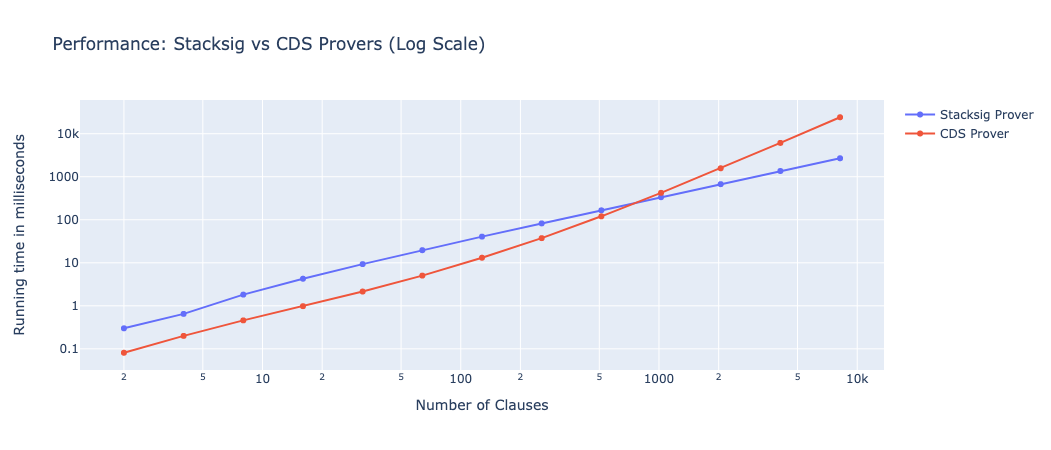
\includegraphics[width=0.9\linewidth]{../assets/plots/vs_provers.png}
  \caption{Comparison of CDS94 Prover and Stacking Sigmas Prover Algorithms.}
  \label{fig:provers_vs}
\end{figure}

\begin{figure}[H]
  \centering
  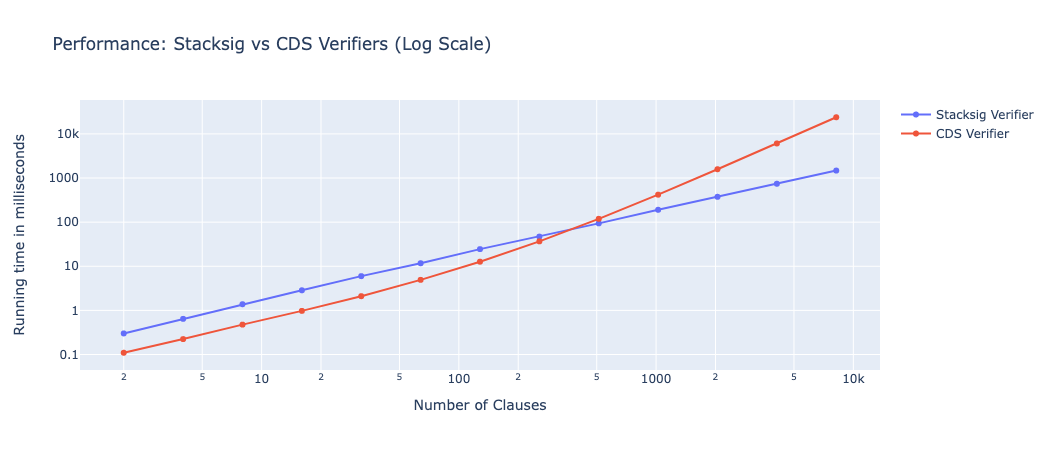
\includegraphics[width=\linewidth]{../assets/plots/vs_verifiers.png}
  \caption{Comparison of the Verifier algorithms of CDS94 and Stacking Sigmas.}
  \label{fig:verifiers_vs}
\end{figure}

These results indicate that if computation speed is the priority,
 it may be more appropriate to use Stacking Sigmas 
when the number of clauses is large (i.e. 512 or more), compared to an implementation of 
CDS94 that uses Lagrange's interpolation \cite{lagrange} with Shamir's secret sharing 
\cite{DBLP:journals/cacm/Shamir79}. That said, this only applies to 1-out-of-n 
disjunctive zero-knowledge, as k-out-of-n disjunctions are not supported by this 
implementation of Stacking Sigmas.

\paragraph{Total Running Time.} Extending this comparison, we now compare the total running time (prover and verifier)
of the three implementations. In Figure \ref{fig:3log}, we see that the total running time of the CDS94 compiler, the Stacking Sigmas compiler, and Mathias Hall-Andersen's 
implementation. We observe that the total running time of the CDS94 compiler and both 
implementations of Stacking Sigmas is similar to what we observe in 
Figures \ref{fig:provers_vs} and \ref{fig:verifiers_vs}. Comparing the two 
Stacking Sigmas implementations, we notice that the running time of Hall-Andersen's 
implementation is better starting from 128 clauses. As mentioned in Section 
\ref{design:qbinding}, this difference in performance is likely due to our 
decision to trade off performance for usability.


\begin{figure}[H]
  \centering
  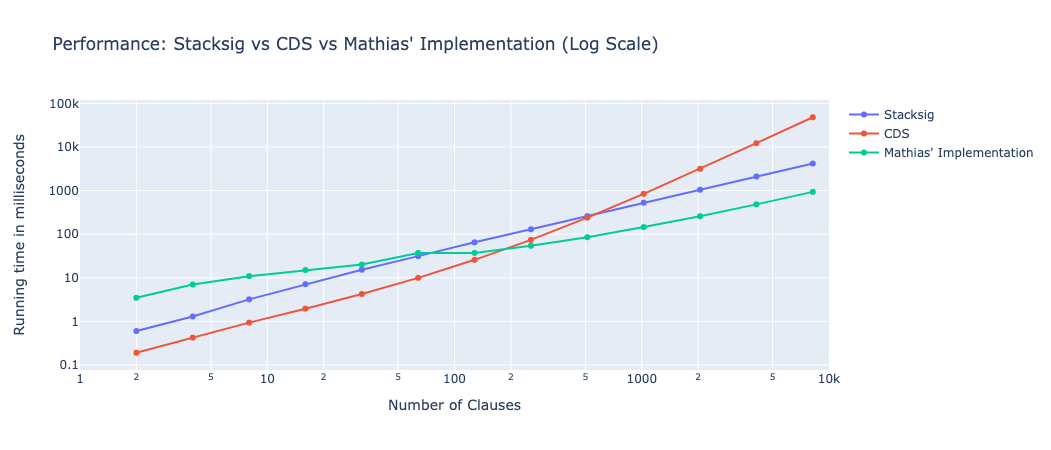
\includegraphics[width=0.9\linewidth]{../assets/plots/3log.png}
  \caption{Comparison of the total running time of the 3 compilers: \cite{CDS94}, 
  Stacking Sigmas \cite{StackingSigmas}, and
  Mathias Hall-Andersen's implementation \cite{MHAStackSig} of Stacking Sigmas.}
  \label{fig:3log}
\end{figure}

 

Our current implementation of the q-binding scheme leads to many calls to the 
\texttt{clone} function which duplicates data. The reason for this is mainly due 
to our lack of experience with Rust and can be improved in future work. Furthermore, 
in Hall-Andersen's implementation, a protocol for every power of two number of 
clauses requires the instantiation of a new type. This means that 
a disjunction of 2 clauses, 4 clauses, 8 clauses, and so on, must use a different 
type. This is not ideal as it requires the developer to write a lot of boilerplate
code, and also results in code duplication. For this reason,
we believe that the trade-off is sound as it allows for a more usable interface for 
developers and can be further improved. Moreover, this performance difference does 
not affect the correctness of the implementation or the goal of our benchmarks. 


\paragraph{CDS94 with an increase in Active Clauses.} Finally, we plot the running time of the CDS94 prover and verifier as the number of
\textbf{active clauses} increase (every power of 2 from 1 to 512 active clauses). 
For this benchmark, we fix the total number of clauses to 512.

\begin{figure}[H]
  \centering
  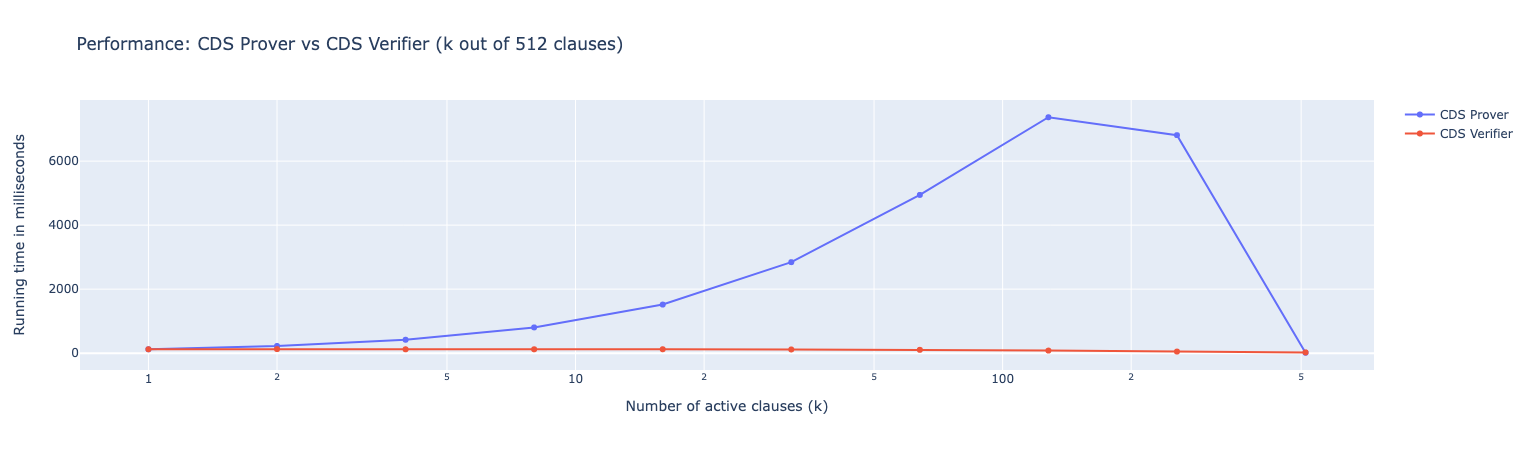
\includegraphics[width=\linewidth]{../assets/plots/cds_threshold.png}
  \caption{Comparison of prover and verifier algorithms as \textit{active clauses} increase. Note that the $x$-axis is on the logarithmic scale.}
  \label{fig:cds_threshold}
\end{figure}

In Figure \ref{fig:cds_threshold}, we see that the
prover running time peaks at 128 clauses, and drops abruptly at 512 clauses. Meanwhile, 
the verifier running time is constant as expected because the number of active clauses does not affect the verifier algorithm -- only the total number of clauses does.
The behaviour of the prover's running time can be directly attributed to 
our \textsf{Complete} algorithm (Definition \ref{def:sss-completion})
which we show in Listing \ref{lst:sss-completion}.

When completing the shares for the active clauses, we are required to interpolate 
at the point corresponding to the index of the active clause (this is the \texttt{x}
variable in the code listing). This interpolation 
uses the secret and the maximally unqualified set of shares to obtain the 
polynomial. As mentioned earlier, Lagrange's polynomial interpolation is an 
$O(n^2)$ algorithm, where $n$ is the number of points used to interpolate. 
Furthermore, the interpolation algorithm is called $k$ times where $k$ is the number of active 
clauses. This means that $n = \texttt{total clauses} - k + 1$. 

\begin{lstlisting}[language=rust, caption={Share Completion Algorithm},label={lst:sss-completion}]
  let remaining_shares = remaining_xs
      .iter()
      .map(|x| {
          let y = poly.interpolate(*x);
          Share { x: *x, y }
      })
      .collect();
\end{lstlisting}

Hence, the total running time of the \textsf{Complete} algorithm is $O(k \cdot n^2)$ (or
$g(k) = k \cdot (513 - k)^2$ in our case). By plotting function $g$ as a graph, we observe a 
direct correlation with what we observe in Figure \ref{fig:cds_threshold}. This is 
easy to see if we show this function as a table:

\begin{table}[H]
  \centering\caption{Active clauses \& $g(k)$}
  \vspace{0.5em}
  \begin{tabular}{lll}
    \toprule
    \textbf{Active Clauses} & \textbf{Threshold} & \textbf{$g$} \\
    \midrule
    1  & 512  & $262144$  \\
    2  & 511  & $522242$  \\
    4  & 509  & $1036324$  \\
    8  & 505  & $2040200$  \\
    16 & 497  & $3952144$ \\
    32 & 481  & $7403552$ \\
    64 & 449  & $12902464$ \\
    128 & 385 & $18972800$\\
    256 & 257 & $16908544$ \\
    512 & 1   & $512$ \\
    \bottomrule
  \end{tabular}
\end{table}

These results shed light on the effects of using Lagrange's polynomial interpolation algorithm 
with Shamir's secret sharing scheme. The CDS94 compiler \cite{CDS94} with Shamir's Secret Sharing 
and Lagrange's interpolation is most effective when the number of active clauses matches the 
total number of clauses. However, this is arguably an uninteresting case as it is no different to 
a \textit{conjunction} of clauses requiring the verifier to check every clause. In practice, we 
expect the number of active clauses to be in a smaller range. This indicates that Lagrange's 
interpolation algorithm is not the most ideal algorithm for Shamir's secret sharing scheme, 
as the running time increases cubically with the number of active clauses until it peaks 
at two powers of 2 below the total number of clauses.

\subsection{Summary of Results}
To summarise, we have first verified the proofs regarding the communication size of each 
compiler as the results here are consistent with the results in the literature 
\cite{CDS94,StackingSigmas}. 

Next, we have revealed important insights into the performance 
of the CDS94 and Stacking Sigmas compiler. It is clear that our implementation of the 
CDS94 compiler is significantly faster than the Stacking Sigmas compiler when the number of 
clauses is small. That said, the Stacking Sigmas compiler has a communication size that 
grows logarithmically with the number of clauses, while the CDS94 compiler's communication
size grows linearly. Hence, a trade-off has to be made between the need for a smaller 
communication size and the need for a faster computation time. 

In general, we believe that 
the Stacking Sigmas compiler is more suitable in any use case where a 1-out-of-n disjunctive proof is suitable. This is primarily because of the large savings 
in communication size (kilobytes of data) and the small increase in computation time 
(a few milliseconds) of using it when the number of clauses is small. When the number of 
clauses increases, CDS94 performs worse and the performance degradation is far more significant 
because of the large number of clauses. For use cases where a k-out-of-n threshold proof is 
required, the CDS94 compiler has to be used. Further improvements could be made to 
our implementation of CDS94 to further reduce computation time and improve performance 
as the number of active clauses or the total number of clauses increase. This will be interesting 
to explore in future work. 

\section{Limitations}\label{sec:limitations}
Despite achieving our primary objectives for this project, we had initially planned for this project to be more comprehensive and complete. Within our progress report (Chapter \ref{ch:progress-report}), we had initially planned to conduct basic security testing on our software using techniques such as fuzzing and static analysis. This is outlined in Section \ref{sec:security_testing}. However, due to delays in software development mainly due to difficulties in fixing bugs related to correctness, this became infeasible within our time constraints. As a result, our efforts toward security come only in the form of threat modelling and simple static analysis. With more time, more robust and comprehensive tests should be performed to fine-tune our implementation. Additionally, our implementation of the q-binding scheme is currently far from ideal and will require further improvements. As mentioned in previous sections, the two main issues are with the performance overhead and the mistake in our implementation for the case of a disjunction of 2 clauses. The latter is to be prioritised as it directly relates to the correctness of our implementation. 